\documentclass[conference]{IEEEtran}

\usepackage{cite}
\usepackage{amsmath,amssymb,amsfonts}
\usepackage{algorithmic}
\usepackage{graphicx}
\usepackage{textcomp}
\usepackage{xcolor}
\usepackage{verbatim}
\usepackage[brazilian]{babel}
\usepackage[utf8]{inputenc}
\usepackage[T1]{fontenc}

% \def\BibTeX{{\rm B\kern-.05em{\sc i\kern-.025em b}\kern-.08em
%     T\kern-.1667em\lower.7ex\hbox{E}\kern-.125emX}}
\begin{document}

\title{Aplicação de Filtros para Estabilização de Controle VR}
%\title{Análise Comparativa da Filtragem da Orientação do Controle Gear VR}
%\title{Visualização do Filtro de Kalman na Estabilização de Controle para Realidade Virtual}

\author{\IEEEauthorblockN{Thiago Figueira\IEEEauthorrefmark{1},
Adriano Gil\IEEEauthorrefmark{1}}
\IEEEauthorblockA{\IEEEauthorrefmark{1}Samsung Instituto de Desenvolvimento para a Informática da Amazônia\\
SIDIA,\\
Manaus -- AM -- Brazil}}

\maketitle

\begin{abstract}
Virtual reality applications make use of multiple sensors in order to translate actions performed by the user on the real world into the virtual environment. The joystick is the main form of interaction and as a sensor, is also subject to noises thus worsening the user experience. This paper compares three different filters applied to a noisy VR controller in a application in Unity3D seeking improvements to user perception and responsiveness.
\end{abstract}

\begin{IEEEkeywords}
virtual reality, games, filters
\end{IEEEkeywords}

%Reescrever mais
\section{Introdução}
% 1. Contextualizar o problema
Jogos e aplicações de realidade virtual utilizam \textit{hardware} especial para permitir a interação do usuário através de sensores inerciais - tais quais o acelerômetro, giroscópio e magnetômetro - os quais mensuram orientação, aceleração, taxa angular, campos magnéticos e essencialmente traduzem um evento na realidade do usuário para seu correspondente no cenário virtual. Contudo, as informações de interesse são suscetíveis a ruídos, isto é, o valor avaliado não reflete plenamente a legítima condição do sistema no momento da medição.

% * Definição introdutória de Filtros
Portanto, este trabalho compara a acurácia entre os filtros de kalman, passa-baixa e adaptativo em uma aplicação de realidade virtual construída em \textit{Unity} que faz uso do controle do Samsung \textit{Gear VR} com a intenção de determinar as diferenças entre cada um deles e apontar o filtro ideal para uso em sistemas VR (\textit{virtual reality}, realidade virtual).

% * Estrutura do artigo
A seção \ref{sec:relatedworks} explora outros trabalhos que abordam o uso de filtros e sensores. Uma breve definição dos filtros é revisada na seção \ref{sec:filters}. O controle de realidade virtual da Samsung é descrito na seção \ref{sec:vrcontroller}. A implementação proposta é detalhada na seção \ref{sec:viztool} e seus resultados são discutidos na seção \ref{sec:results}. Por fim, enumeram-se as conclusões e perspectivas de trabalhos futuros na seção \ref{sec:conclusion}.

\section{Trabalhos Relacionados} \label{sec:relatedworks}

% Alguns exemplos de aplicações
Entre alguns exemplos de emprego do Filtro de Kalman: \cite{demkowiczkalman} demonstra uma aplicação Java do filtro em sistemas sondadores de multi-feixe para remover ruído na visualização 3D do fundo do mar, onde os dados de entrada são filtrados duas vezes em diferentes orientações. \cite{choset2005principles} mostra a eficácia do filtro de Kalman no uso de sistemas de navegação de robôs, pois normalmente o conhecimento de mundo deste robô deriva de medidas fornecidas por sensores ruidosos.

Alguns artigos trabalham com a filtragem de sensores baseados em acelerômetro: \cite{schlomer2008gesture} usa o modelo oculto de Markov para reconhecimento de gestos do usuários feitos em um \textit{Wiimote}, o controle do \textit{Wii}, a filtragem ocorre por meio de filtros simples para remover pontos que não são suficientemente significantes. \cite{shiratori2008accelerometer} utiliza múltiplos controles de \textit{Wii} para criar animações procedurais, as informações do acelerômetro são analisadas e aplica-se o filtro de Kalman para remover o ruído  gerado pelo movimento.

Apesar destes estudos, \cite{VRDataGlove} é um trabalho em progresso que reporta um estudo de usabilidade que visa determinar a efetividade entre dois tipos de entrada para realidade virtual: controle e gestos de mão. 

\begin{comment}
\section{Unity3D} \label{sec:unity3d}
Também alcunhado por \textit{Unity}, trata-se de um ambiente de desenvolvimento (com \textit{engine} gráfica e editor de código) desenvolvido pela \textit{Unity Technologies}. Fornece uma plataforma para a criação de jogos e aplicativos em duas ou três dimensões, além de realidade aumentada e virtual para o público de computadores, dispostivos móveis, consoles, web e sistemas integrados ou HDM (\textit{head-mounted displays}). 
\end{comment}

\section{Filtragem da Orientação do Controle} \label{sec:filters}
Sensores têm a finalidade de quantificar comportamentos ou características da realidade através de transdutores que convertem a energia de entrada em energia de saída. Neste processo, registra-se uma amostra do evento de interesse, isto é, processa-se uma série de capturas da realidade de maneira a converter a medida de interesse em um conjunto contínuo de valores. Este procedimento, contudo, está suscetível a erros, seja devido à natureza física do transdutor que não traduz fielmente os valores medidos, seja na insuficiência dos dados capturados pela amostragem, ou ainda na discretização dos valores contínuos da realidade. Somadas estas possibilidades, percebe-se que as informações de interesse (velocidade, orientação, localização no GPS, etc.) são suscetíveis a ruídos, isto é, o valor medido não reflete em sua totalidade a verdadeira condição do sistema no momento da medição.

Desta forma, a fim de garantir o maior nível de aproximação no que se refere à confiabilidade das informações tratadas, os filtros tornam-se ferramentas preciosas as quais visam garantir que os dados relevantes sejam observados. Este trabalho apresenta o uso do controle de \textit{Gear VR} sem filtragem e com filtragem através três filtros: kalman, passa-baixa e adaptativo, a fim de determinar qual deles é mais apropriado para uso, tendo em vista que fatores como responsividade e precisão são cruciais para a imersão em uma aplicação de realidade virtual \cite{VRDataGlove}.

Apresentado no ano de 1960 pelo criador de mesmo nome, o filtro de Kalman descreve de uma solução recursiva para o problema de filtragem de dados em um sistema dinâmico linear \cite{WelchBishop}, isto é, trata-se de um sistema capaz de predizer um estado futuro baseado nas últimas informações disponíveis. Descrito como um sistema de recursivo de predição ótima, o filtro de Kalman é efetivamente utilizado em muitas aplicações do mundo real, uma delas foi a própria viagem do homem à Lua, quando necessitava-se estimar as trajetórias para a ida e volta deste satélite \cite{GrewalAndrews}.

O filtro passa-baixa permite a passagem de baixas frequências, mas suaviza a amplitude de frequências acima da frequência de corte.

\section{Controle para Realidade Virtual} \label{sec:vrcontroller}

% * Qual a importância/valor de usar controles?
Aplicativos de realidade virtual normalmente são executados dentro de óculos especialmente feitos para a renderização de duas telas, uma para cada olho, conferindo assim a ilusão de profundidade em um universo virtual, maximizando a imersão do usuário. Em aplicações de realidade virtual, normalmente o controle posiciona um cursor que representa o foco de interação do usuário.

% * Tipos de Controles
Há variações no que se refere às capacidades dos diferentes tipos de controle, o próprio headset, i.e. o equipamento de realidade virtual vestível, possui um controle baseado no giroscópio; existem também controladores que fornecem informações posicionais, permitindo um maior nível de liberdade para o usuário, visto que há a possiblidade de manipulação de diferentes elementos, além da movimentação do próprio personagem do usuário.

% * Descrever controle da Samsung
A figura \ref{figure:vrcontroller} mostra o controle que acompanha o óculos de realidade virtual \textit{GearVR SM-R324} da Samsung. A \textit{Oculus} é atualmente parceira da Samsung na distribuição de soluções para realidade virtual através de dispositivos móveis e disponibiliza um \textit{SDK} para uso de funcionalidades específicas em aplicações de realidade virtual, dentre elas uma API para captação dos dados de rotação do controle \cite{gearvrinputdocs}.

\begin{figure}[h!]
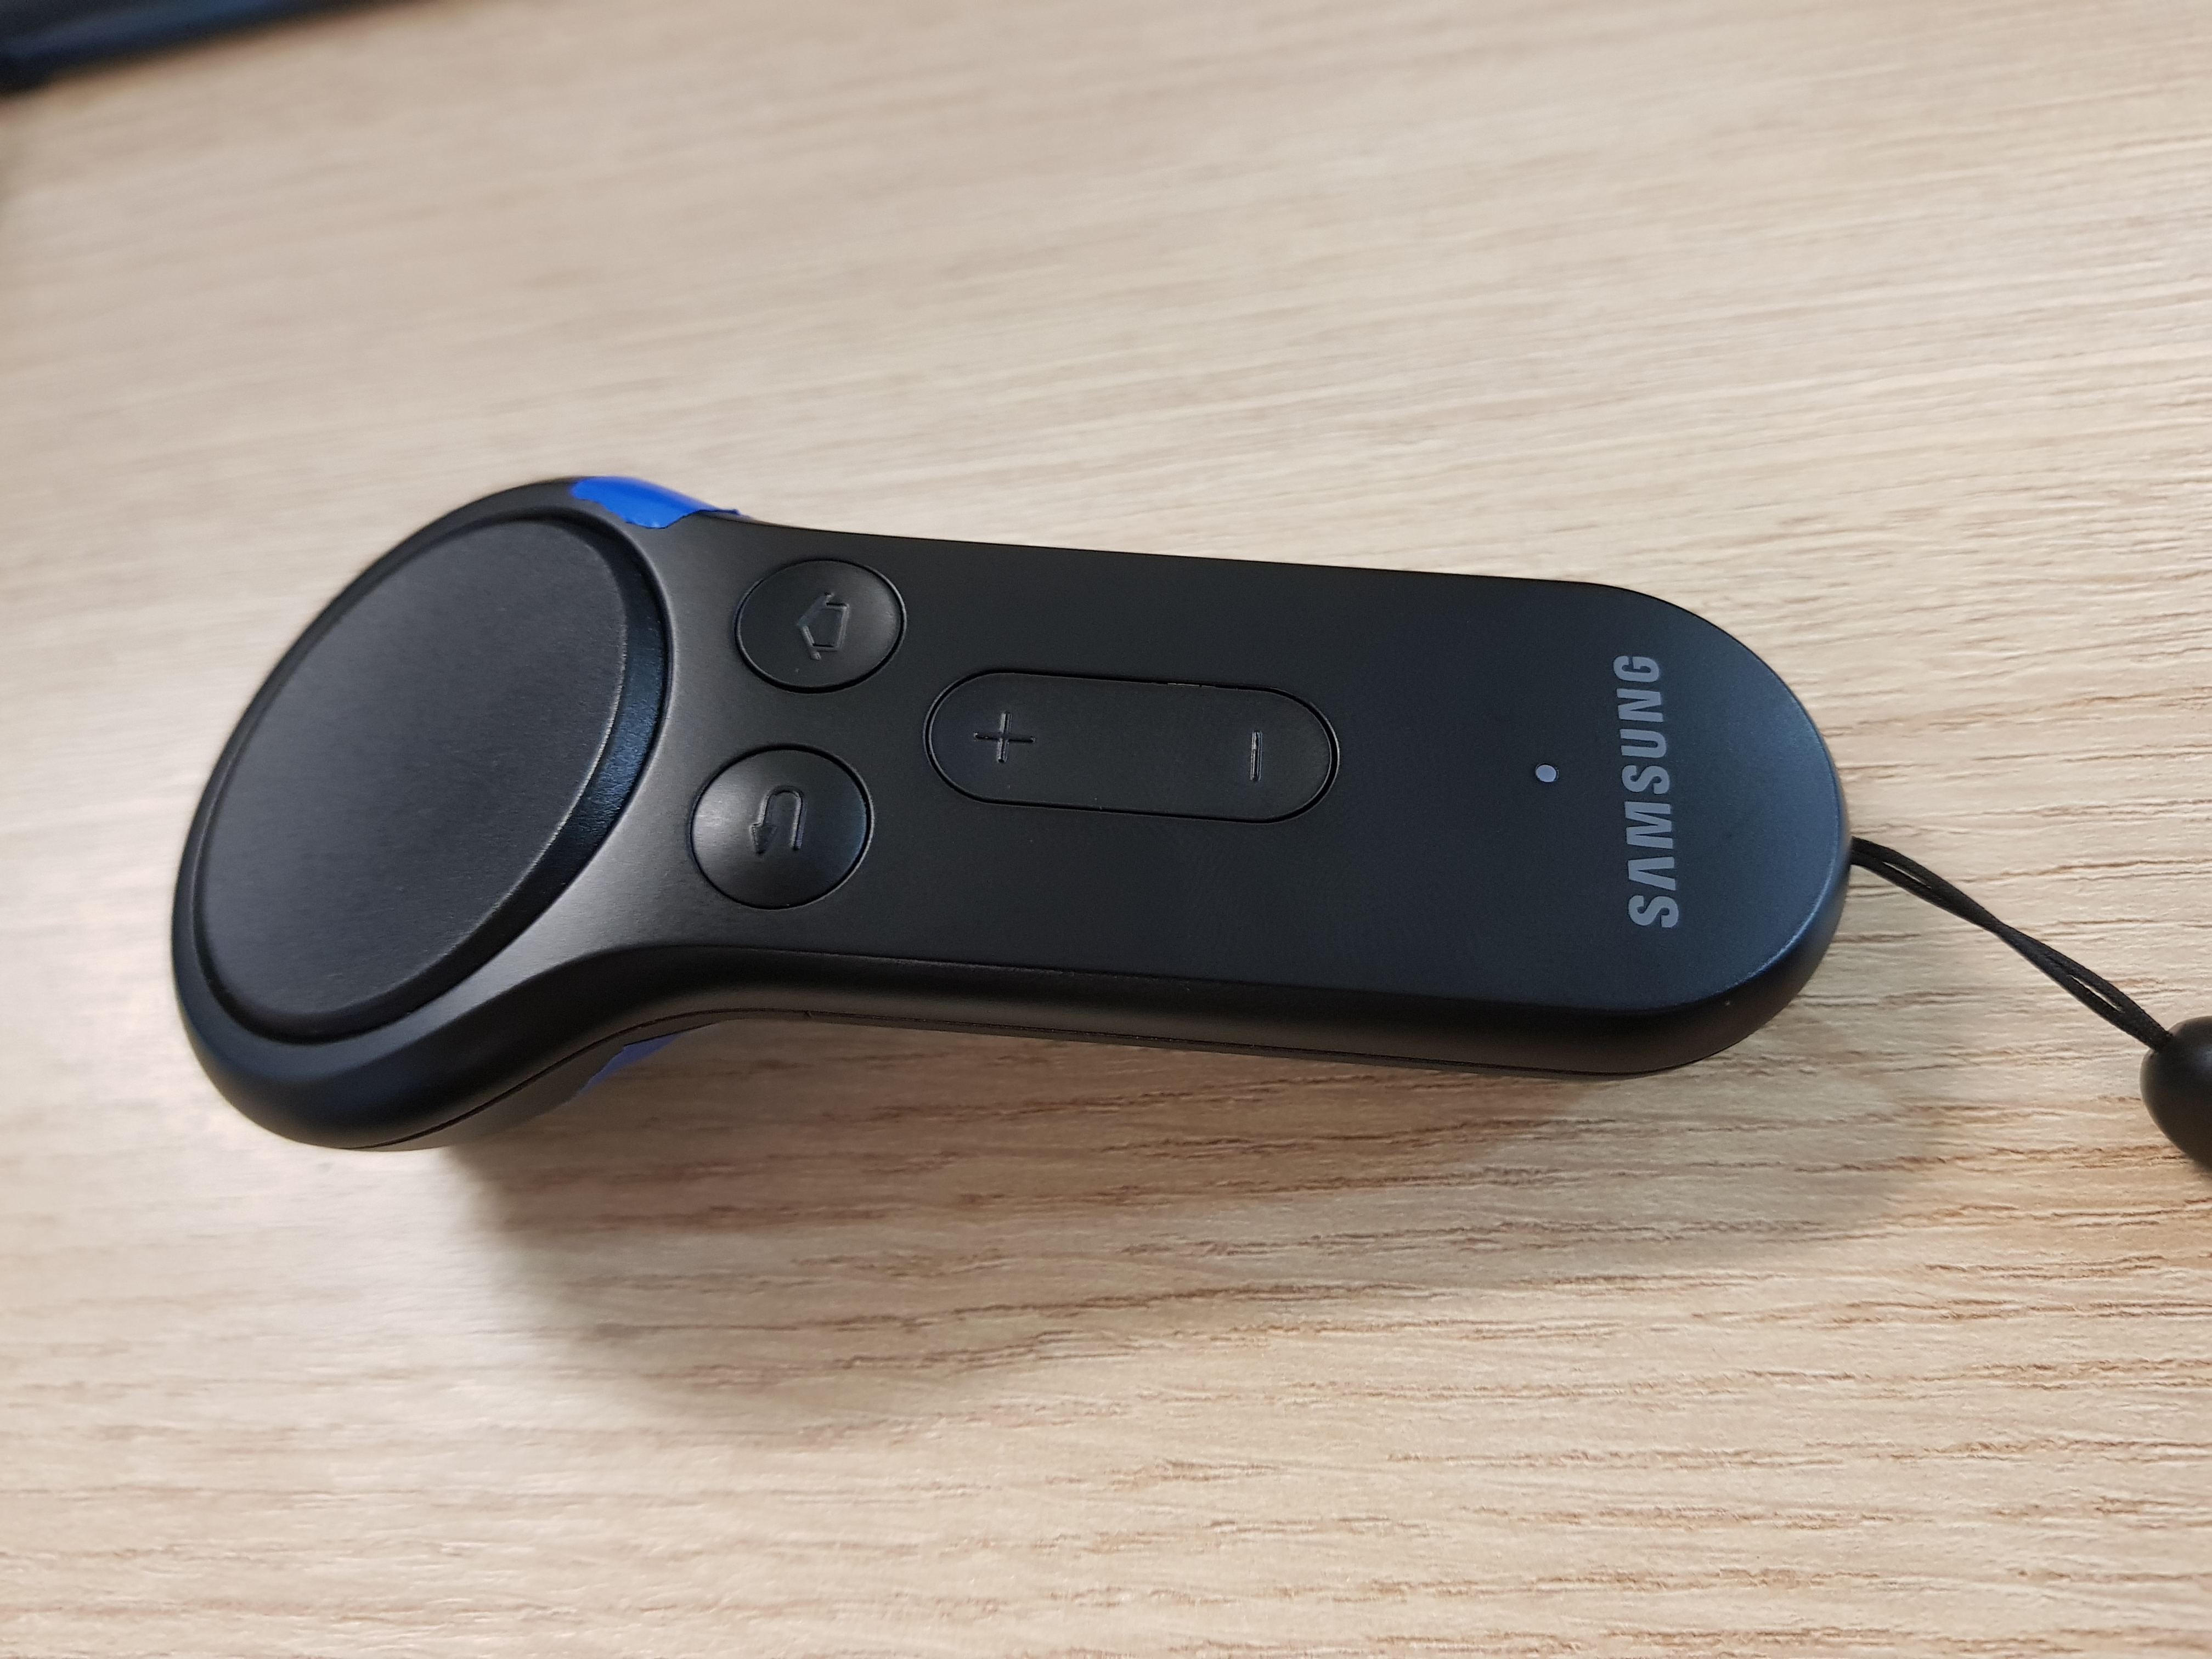
\includegraphics[width=\linewidth]{images/gear_controller.jpg}
\caption{Controle para Realidade Virtual da Samsung.}
\label{figure:vrcontroller}
\end{figure}

\section{Ferramenta de Visualização de Filtros} \label{sec:viztool}

% Proposal
Este artigo se propõe a implementar uma ferramenta para a visualização do emprego do filtro de Kalman na estabilização de um controle de realidade virtual. O uso do filtro é motivado pela necessidade de remoção dos ruídos de leitura e obtenção de um controle mais estável para o usuário. A contribuição para o desenvolvedor é a capacidade de visualizar o efeitos do ruído e compreender como este pode ser amenizado pelo uso do filtro de Kalman; para o usuário final, a criação de um componente para controle de realidade virtual que possibilite movimentos mais precisos.

% As a didatic tool
Dado o objetivo de remover ruídos de um conjunto determinado de sinais, é de grande interesse para o desenvolvedor assimilar de que forma este ruído potencialmente afeta uma aplicação em realidade virtual: principalmente através da geração de um cursor mais trêmulo, menos responsivo ou confiável, dificultando, portanto, a experiência do usuário.

% Describe Unity implementation - Noise visualization
Para visualizar o ruído, utilizou-se elementos de partículas ou \textit{ParticleSystem} para renderizar pontos onde o cursor deveria estar levando em conta as entradas ruidosas tais como recebidas pelo controle. As partículas geradas foram configuradas para ter uma cor destoante, uma tonalidade de vermelho indica a entrada real obtida pelo controle e, ao longo do tempo, reduz-se a luminosidade das partículas de modo a adicionar uma informação temporal à visualização gerada. Assim, pontos vermelhos mais vivos indicam os dados mais recentes recebidos pelo controle enquanto pontos mais fracos representam posições mais antigas.

Afim de comparar a entrada ruidosa e o resultado filtrado, as posições filtradas pelo filtro de Kalman foram destacadas em azul, através de \textit{TrailRenderer} que permite renderizar o caminho percorrido pelo cursor ao longo da execução da aplicação.

\begin{figure}[h!]
\centering
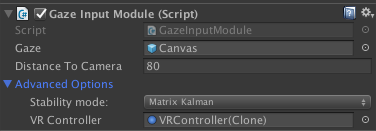
\includegraphics[width=\linewidth]{images/controller_input.png}
\caption{Componente Unity para configuração do controle da Samsung.}
\label{fig:controllercomponent}
\end{figure}

% Describe Unity implementation - GearVRInput component
Implementamos um componente de gerenciamento de entradas do usuário chamado \textit{GazeInputModule}, permitindo mudar o cursor de acordo com a posição da cabeça do usuário fornecida pelo \textit{headset GearVR} ou pela rotação do controle.

% Describe interaction with controller
O controle de realidade virtual da Samsung, tal como descrito na seção \ref{sec:vrcontroller}, possibilita obter dados de rotação em tempo real \cite{gearvrinputdocs} na forma de um \textit{quaternion} \cite{quaternionhamilton1844ii} que representa a orientação atual do dispositivo. \textit{Quaternions} são um sistema numérico que estendem os números complexos e são utilizados por muitas \textit{APIs} gráficas para representar valores de rotação. O \textit{Software Development Kit} SDK da \textit{Oculus} permite obter a rotação em coordenadas angulares (ângulos de Euler). Para cada valor angular é calculado um ponto do cursor que intercepta uma esfera de tamanho unitário e um raio partindo da representação virtual do controle.

\section{Resultados} \label{sec:results}

\begin{figure}[h!]
\centering
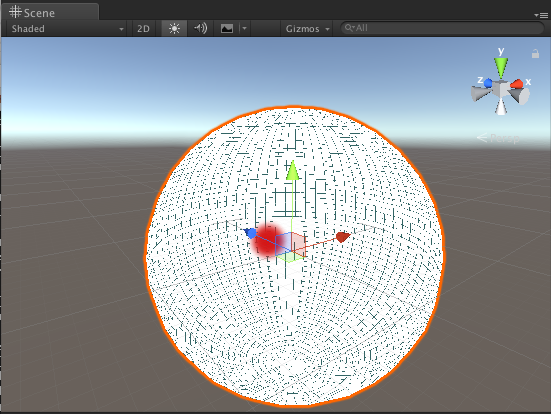
\includegraphics[width=\linewidth]{images/sphere.png}
\caption{Esfera invertida na cena da Unity.}
\label{fig:invertsphere}
\end{figure}

A implementação em Unity3D foi executada em um aparelho Samsung S8 acoplado ao óculos \textit{GearVR SM-R324}. Utilizou-se o controle oficial da Samsung, que acompanha o óculos de realidade virtual \textit{GearVR}. Para fins de teste, foi gerada uma esfera invertida e um código em \textit{shader} para exibir \textit{grids} na superfície da esfera gerando um ambiente branco de cor sólida e sem efeitos de iluminação, tal como exibida na figura \ref{fig:invertsphere}.

Toda aplicação \textit{GearVR} distribuída na \textit{Oculus Store} \cite{gearvrstore} pode ser executada nos modelos de celulares Samsung mais avançados, quando acoplado a um óculos \textit{GearVR}. A qualquer momento durante a execução da aplicação, é possível acessar um menu de opções que permite registrar \textit{screenshots} ou gravar vídeos da experiência vivida pelo usuário no mundo virtual estabelecido pela aplicação.

\begin{figure}[h!]
\centering
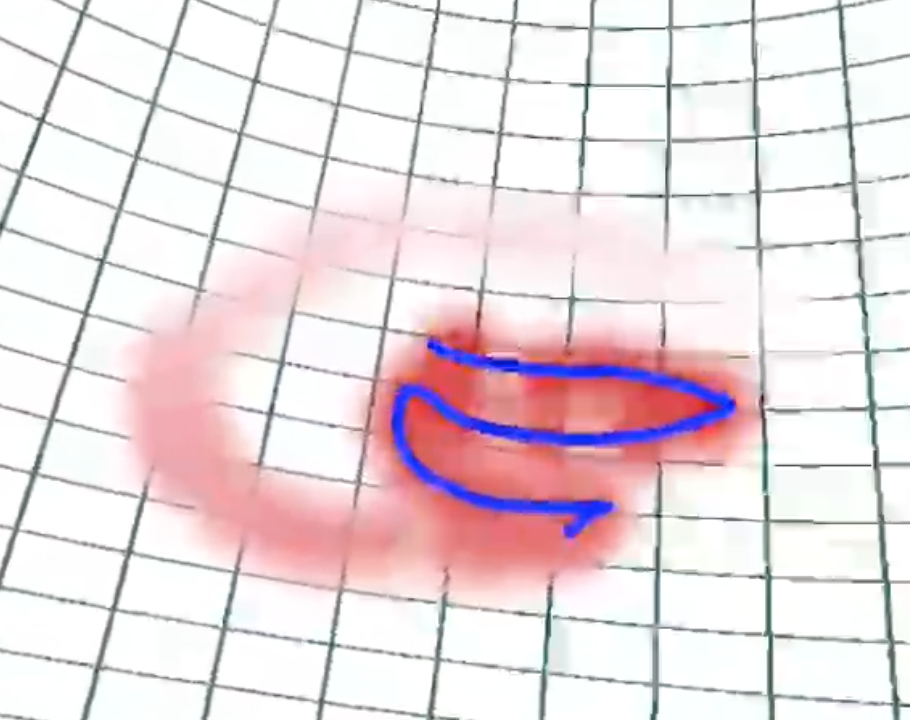
\includegraphics[width=\linewidth]{images/image_01.png}
\caption{Filtragem do cursor de VR. Amostras ruidosas em vermelho e valor filtrado em azul.}
\label{fig:filter01}
\end{figure}

A figura \ref{fig:filter01} mostra um \textit{screenshot} da aplicação em Realidade Virtual com a filtragem de cursor ativa. O caminho do cursor é definido pela rotação atual do controle do \textit{GearVR}. A posição do cursor é calculada na intersecção de uma esfera de tamanho unitário e a direção atual do controle.

\begin{figure}[h!]
\centering
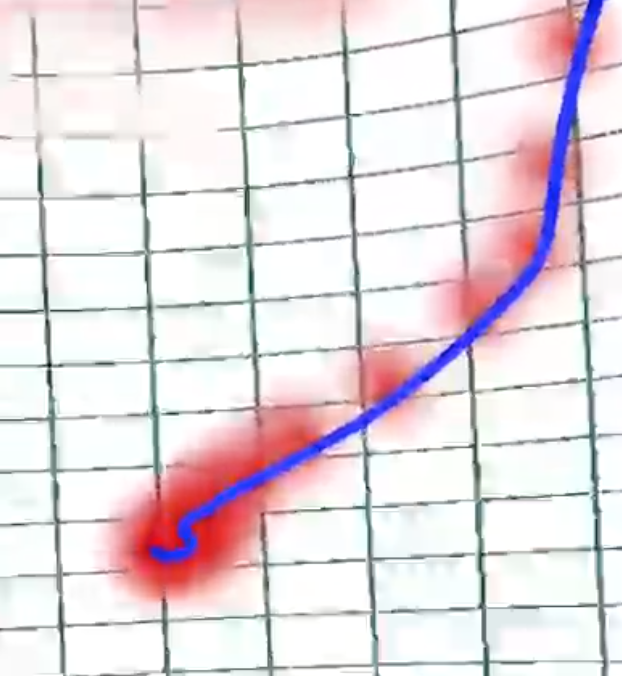
\includegraphics[width=\linewidth]{images/image_02.png}
\caption{Filtragem do cursor de VR. Amostras ruidosas em vermelho e valor filtrado em azul.}
\label{fig:filter02}
\end{figure}

Durante a execução da aplicação, percebeu-se que quando a movimentação do cursor é mais veloz que a taxa de atualização, i.e., o \textit{update}, os pontos de ruído não são visualizados de maneira contínua, provocando o efeito visto na figura \ref{fig:filter02}, onde as partículas concentram-se em apenas alguns pontos amostrados pelo \textit{framerate} da aplicação \textit{Unity}, gerando regiões ruidosas espaçadas entre si.

Na figura \ref{fig:filter01} e \ref{fig:filter02} verifica-se que a linha azul forma-se de maneira estável ao longo do caminho percorrido pelo cursor, enquanto os pontos vermelhos se espalham ao redor desse caminho, indicando que a amplitude máxima de instabilidade é cerca de duas vezes maior que o tamanho do cursor, ou seja, facilmente perceptível pelo usuário e que impossibilitaria a realização de movimentos precisos e estáveis, em outras palavras, a exatidão e responsividade esperadas do controlador não são satisfatórias.

\section{Conclusão} \label{sec:conclusion}

Apresentou-se neste artigo uma implementação do filtro de Kalman para estabilização do controle de realidade virtual da Samsung. Concomitantemente, descreveu-se a visualização das entradas ruidosas fornecidas pelo controle e o efeito resultante após a aplicação do filtro de Kalman. Afim de estimular a reutilização da implementações feitas, foram gerados componentes para rápida configuração, tal como demonstrado na figura \ref{fig:controllercomponent}.


Através resultados obtidos, verificou-se que a solução desenvolvida em \textit{Unity} foi capaz de filtrar as posições ruidosas geradas pelo controlador e garantir um nível de controle mais estável em aplicações de realidade virtual. Implementou-se também uma ferramenta para visualização da filtragem de entradas ruidosas.


Em trabalhos futuros propõe-se estender a aplicação do filtro à problemas de outras naturezas, tais quais em aplicações onde haja \textit{jittering} na movimentação de personagens ou ainda em aplicações de realidade aumentada para os mais diversos fins, como garantir que a movimentação de um \textit{non-playable character} (NPC) seja a mais suave possível.


Fora do campo da aplicações digitais, há muitos exemplos possíveis para a aplicação:  um pequeno robô de jardim que precisa saber sua verdadeira localização a fim de evitar quedas; um mapa de navegação para carros que, dentro de um túnel, precise cumprir sua função com precisão para guiar o motorista; ou ainda, a necessidade de conhecer-se a temperatura de um foguete cujo alto aquecimento impeça a medição direta através de um sensor. Se analisadas com cadência, as situações ilustradas possuem em comum a existência de informações que são passíveis de ruídos ou imprecisão os quais podem ser minimizados com o uso do filtro de Kalman.

\begin{comment}
\section*{Acknowledgment}
The preferred spelling of the word ``acknowledgment'' in America is without 
an ``e'' after the ``g''. Avoid the stilted expression ``one of us (R. B. 
G.) thanks $\ldots$''. Instead, try ``R. B. G. thanks$\ldots$''. Put sponsor 
acknowledgments in the unnumbered footnote on the first page.
\end{comment}

\bibliographystyle{IEEEtran}
\bibliography{references}

% \begin{thebibliography}{00}
% \bibitem{b1} G. Eason, B. Noble, and I. N. Sneddon, ``On certain integrals of Lipschitz-Hankel type involving products of Bessel functions,'' Phil. Trans. Roy. Soc. London, vol. A247, pp. 529--551, April 1955.
% \bibitem{b2} J. Clerk Maxwell, A Treatise on Electricity and Magnetism, 3rd ed., vol. 2. Oxford: Clarendon, 1892, pp.68--73.
% \bibitem{b3} I. S. Jacobs and C. P. Bean, ``Fine particles, thin films and exchange anisotropy,'' in Magnetism, vol. III, G. T. Rado and H. Suhl, Eds. New York: Academic, 1963, pp. 271--350.
% \bibitem{b4} K. Elissa, ``Title of paper if known,'' unpublished.
% \bibitem{b5} R. Nicole, ``Title of paper with only first word capitalized,'' J. Name Stand. Abbrev., in press.
% \bibitem{b6} Y. Yorozu, M. Hirano, K. Oka, and Y. Tagawa, ``Electron spectroscopy studies on magneto-optical media and plastic substrate interface,'' IEEE Transl. J. Magn. Japan, vol. 2, pp. 740--741, August 1987 [Digests 9th Annual Conf. Magnetics Japan, p. 301, 1982].
% \bibitem{b7} M. Young, The Technical Writer's Handbook. Mill Valley, CA: University Science, 1989.
% \end{thebibliography}
% \vspace{12pt}
% \color{red}
% IEEE conference templates contain guidance text for composing and formatting conference papers. Please ensure that all template text is removed from your conference paper prior to submission to the conference. Failure to remove the template text from your paper may result in your paper not being published.

\end{document}
